\section{Atenuación de los cuatro medios a 3 GHz}
El agua marina presentó la mayor caída de flujo radial compensado, seguida por el músculo y el concreto (Cuadro~\ref{t:principal}). En concreto, la pendiente ajustada difirió de la referencia en $0.00039$ dB/mm. En músculo la diferencia alcanzó $0.02498$ dB/mm. En vacío se obtuvo una pendiente aparente de $-0.000916$ dB/mm. El perfil compensado creció ligeramente dentro de la ventana estudiada.

\begingroup\small\setlength{\tabcolsep}{4pt}
\begin{longtable}{lrrrrr}
\caption{Atenuación aparente del monopolo a 5 px/mm. Pendientes e intervalos del 95\,\% en dB/mm. El error relativo se calculó respecto de la onda plana.}\label{t:principal}\\
\hline Medio & $\alpha_{\rm app}$ & IC inferior & IC superior & $\alpha_{\rm teo}$ & Error (\%) \\ \hline\endfirsthead
\hline Medio & $\alpha_{\rm app}$ & IC inferior & IC superior & $\alpha_{\rm teo}$ & Error (\%) \\ \hline\endhead
Agua marina & $1.1866$ & $1.1862$ & $1.187$ & $1.2025$ & $1.3248$ \\
Músculo & $0.45718$ & $0.45668$ & $0.45763$ & $0.48216$ & $5.1818$ \\
Concreto & $0.077443$ & $0.077403$ & $0.077481$ & $0.077832$ & $0.49893$ \\
Vacío & $-9.157\times 10^{-4}$ & $-9.375\times 10^{-4}$ & $-8.936\times 10^{-4}$ & $0$ & --- \\
\hline\end{longtable}\endgroup

\begin{figure}[htbp]\centering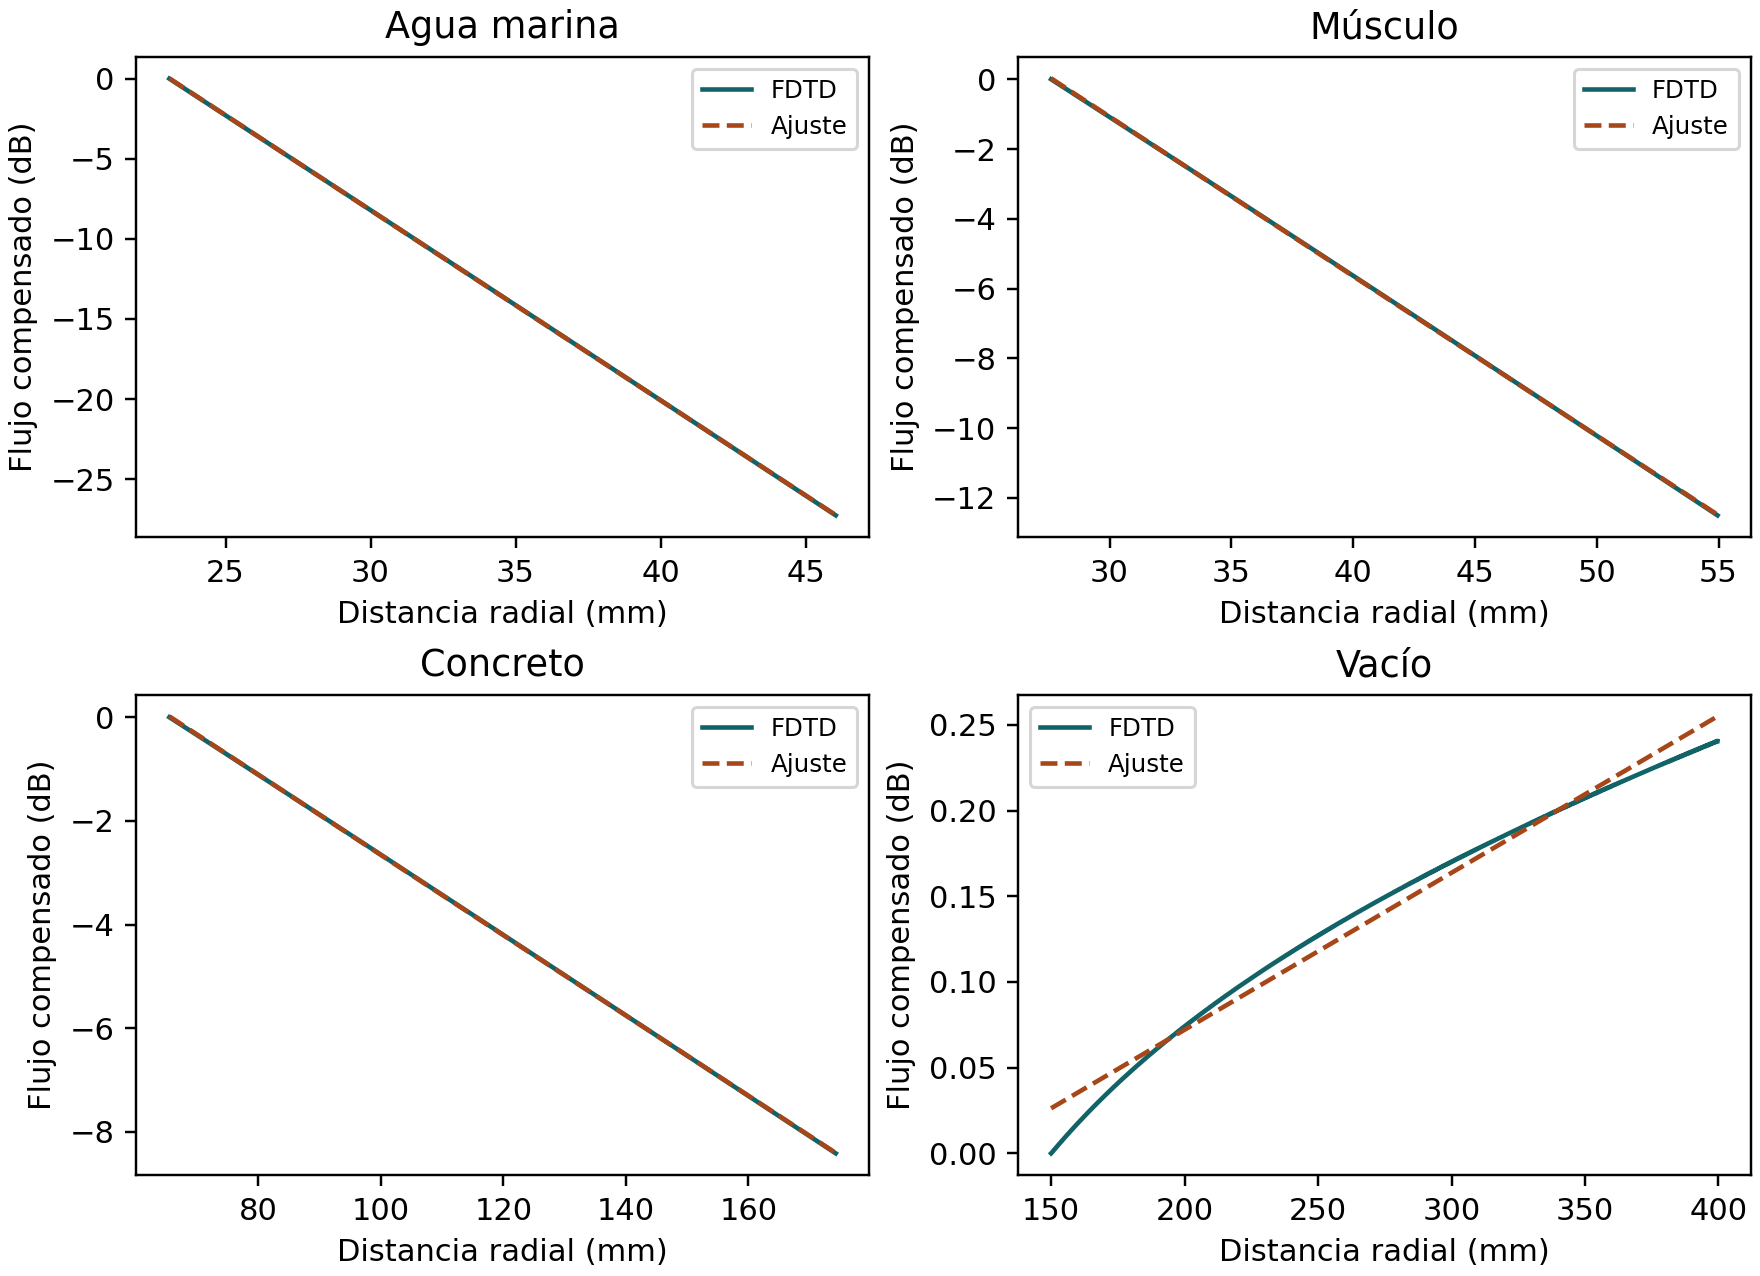
\includegraphics[width=.96\linewidth]{figuras/campana61_perfiles.png}
\caption{Flujo radial compensado en las ventanas de ajuste a 5 px/mm. Cada perfil se normalizó en su primer punto. Las escalas verticales son propias de cada medio.}\label{f:perfiles61}\end{figure}
En la Figura~\ref{f:perfiles61}, las distancias físicas de observación variaron porque la ventana se definió en longitudes de onda del medio. La proximidad visual entre los puntos y las rectas se cuantificó mediante el error cuadrático medio y la dependencia espacial de los residuos (Cuadro~\ref{t:diag}).

\section{Refinamiento y balance local}
La atenuación aparente en agua marina aumentó de 1.18660 a 1.19145, 1.19448 y 1.19624 dB/mm al utilizar 5, 10, 15 y 20 px/mm. La discrepancia frente a la referencia de 1.20253 dB/mm disminuyó del 1.325 al 0.524\,\%. En músculo, al pasar de 5 a 10 px/mm, la pendiente aumentó de 0.45718 a 0.46836 dB/mm. En concreto se obtuvo 0.07746 dB/mm a 10 px/mm. El Cuadro~\ref{t:atte} reúne las estimaciones e intervalos de todas las mallas.

\begingroup\small\setlength{\tabcolsep}{4pt}
\begin{longtable}{lrrrrr}
\caption{Balance del anillo a 5 px/mm. Las potencias se expresaron en unidades de Meep. Las dos últimas columnas se normalizaron por la entrada.}\label{t:balance}\\
\hline Medio & $P_e$ & $P_s$ & $P_J$ & $f_J$ (\%) & $b$ (\%) \\ \hline\endfirsthead
\hline Medio & $P_e$ & $P_s$ & $P_J$ & $f_J$ (\%) & $b$ (\%) \\ \hline\endhead
Agua marina & $2.942\times 10^{-6}$ & $1.796\times 10^{-7}$ & $2.758\times 10^{-6}$ & $93.748$ & $0.14548$ \\
Músculo & $3.731\times 10^{-5}$ & $9.680\times 10^{-6}$ & $2.760\times 10^{-5}$ & $73.984$ & $0.06936$ \\
Concreto & $2.141\times 10^{-4}$ & $1.087\times 10^{-4}$ & $1.054\times 10^{-4}$ & $49.228$ & $0.0038432$ \\
Vacío & $0.0011093$ & $0.0011093$ & $0$ & $0$ & $-2.633\times 10^{-5}$ \\
\hline\end{longtable}\endgroup

En el anillo de agua marina se disiparon 93.75 de cada 100 unidades de potencia entrante a 5 px/mm. En músculo se disiparon 73.98 y en concreto, 49.23. En vacío la disipación de Joule fue cero y la diferencia firmada entre entrada y salida fue $-0.0000263$\,\% de la entrada. El Cuadro~\ref{t:balance} conserva el signo de cada residuo.
\begin{figure}[htbp]\centering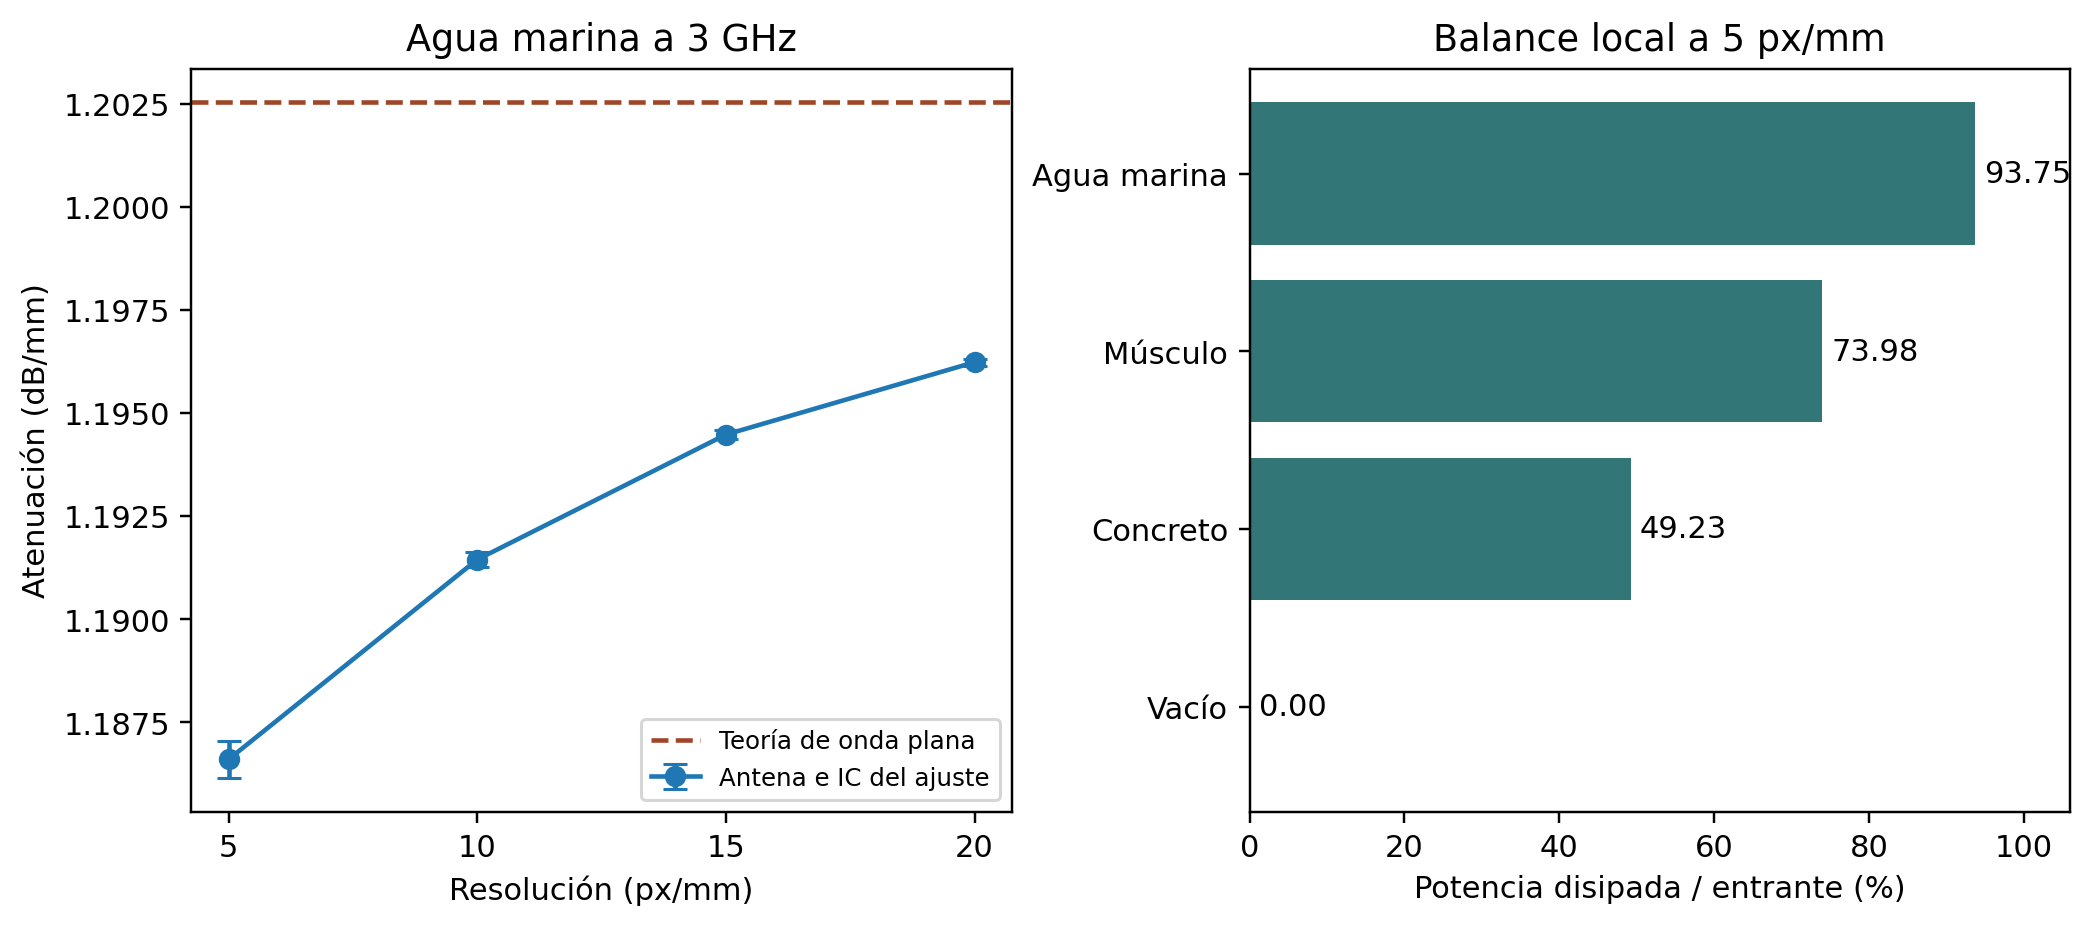
\includegraphics[width=\linewidth]{figuras/campana61_verificacion.png}
\caption{Atenuación aparente en agua marina al refinar la malla y fracción de potencia disipada en el anillo de cada medio. Las barras verticales del primer panel representan el intervalo condicional del ajuste.}\label{f:ver61}\end{figure}

\section{Controles de onda plana e interfaces}
En las ondas planas a 5 px/mm, el error relativo de la pendiente frente a la solución analítica fue 0.0099\,\% en concreto, 0.1452\,\% en agua y 0.1036\,\% en músculo. En vacío, el intervalo del ajuste incluyó cero. Al duplicar la resolución, los errores de los tres medios con pérdidas se redujeron a 0.0025\,\%, 0.0362\,\% y 0.0259\,\%, respectivamente.

En las láminas de 7 mm a 5 px/mm se transmitió el 1.92\,\% de la potencia incidente en agua y el 15.03\,\% en músculo. Las pérdidas de inserción fueron 17.17 y 8.23 dB. En concreto, para el espesor reservado de 30 mm, se transmitió el 36.17\,\% y se obtuvo una pérdida de 4.42 dB. La Figura~\ref{f:lam61} muestra la variación con el espesor. Los Cuadros~\ref{t:lam} y~\ref{t:lamt} incluyen las 41 configuraciones, los valores analíticos y las diferencias firmadas.
\begin{figure}[htbp]\centering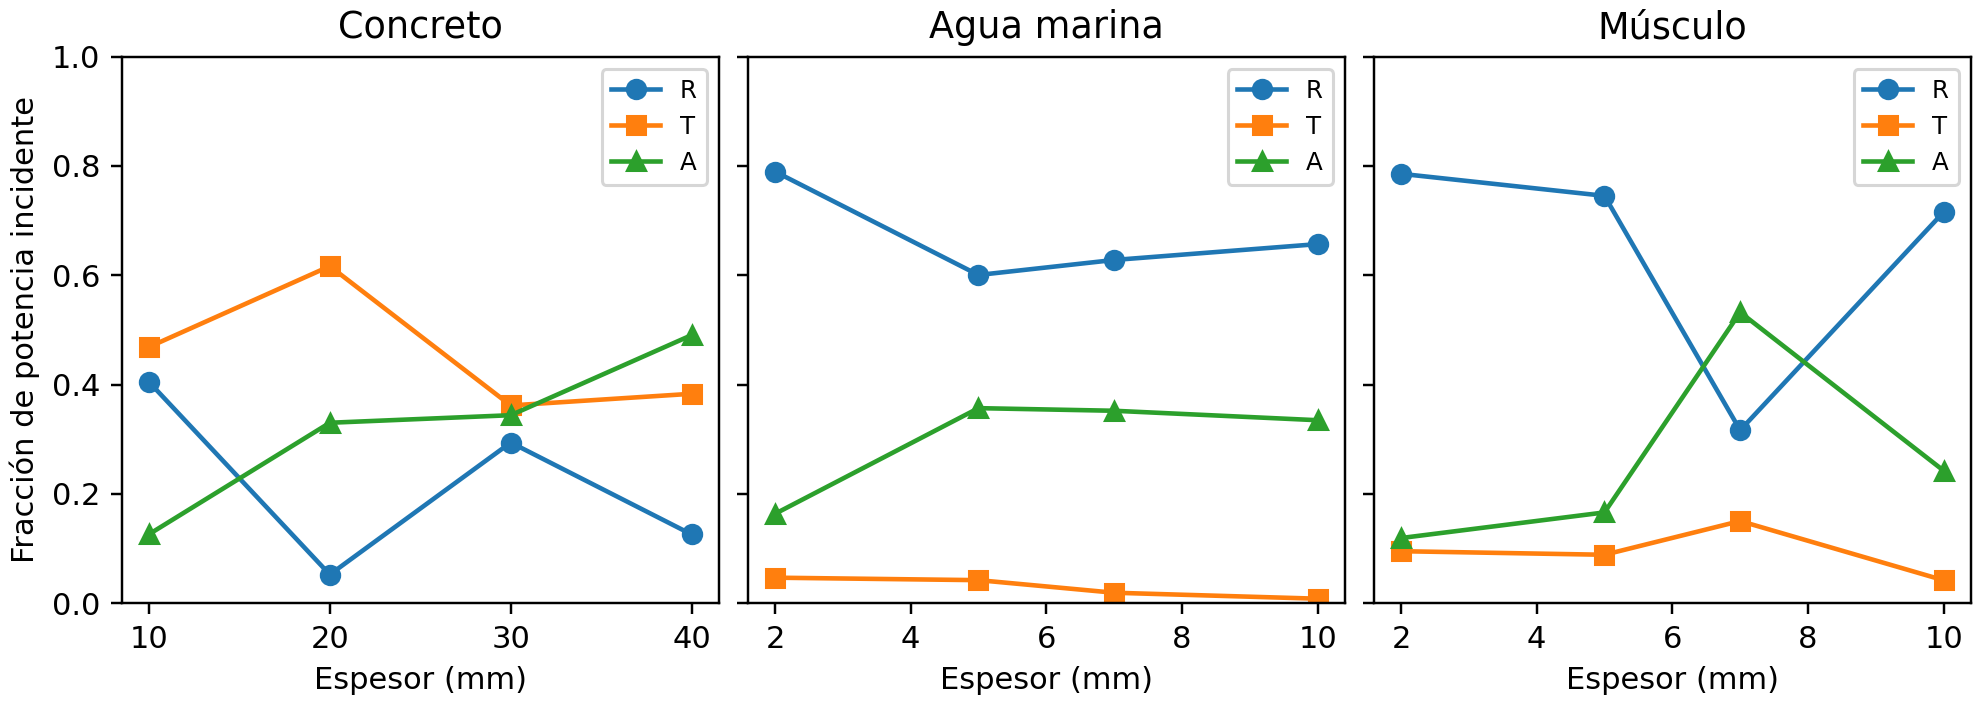
\includegraphics[width=\linewidth]{figuras/campana61_laminas.png}
\caption{Fracciones reflejada ($R$), transmitida ($T$) y absorbida ($A$) a incidencia normal y 5 px/mm. Los símbolos identifican espesores simulados. Las líneas unen puntos del mismo coeficiente.}\label{f:lam61}\end{figure}

El mayor error absoluto observado en un coeficiente fue de 0.1503 puntos porcentuales. Se obtuvo en la absorción del agua a 7 mm y 5 px/mm. El mayor residuo absoluto $100|1-R-T-A|$ de toda la serie fue 0.1087 puntos porcentuales, redondeado hacia arriba.
